\bluepage{Simple video filters in OpenGL}

\begin{frame}[fragile]
\frametitle{RGB to grayscale image}
  {\scriptsize
  \begin{minted}[frame=lines]{glsl}
#version 450

layout(location=0)out vec4 fColor;

layout(binding=0)uniform sampler2D frame;

//texture coordinates
in vec2 vCoord;

uniform uvec2 windowSize = uvec2(1,1);

void main(){
  //read from texture
  vec3 color = texture(frame,vCoord).xyz;

  //convertex to intensity
  float intensity = dot(vec3(.2126,.7152,.0722),color);

  //write intensity to framebuffer
  fColor = vec4(intensity);
}
  \end{minted}
  }
\end{frame}

\begin{frame}
\frametitle{Example - RGB to gray}
  \begin{figure}[h]
  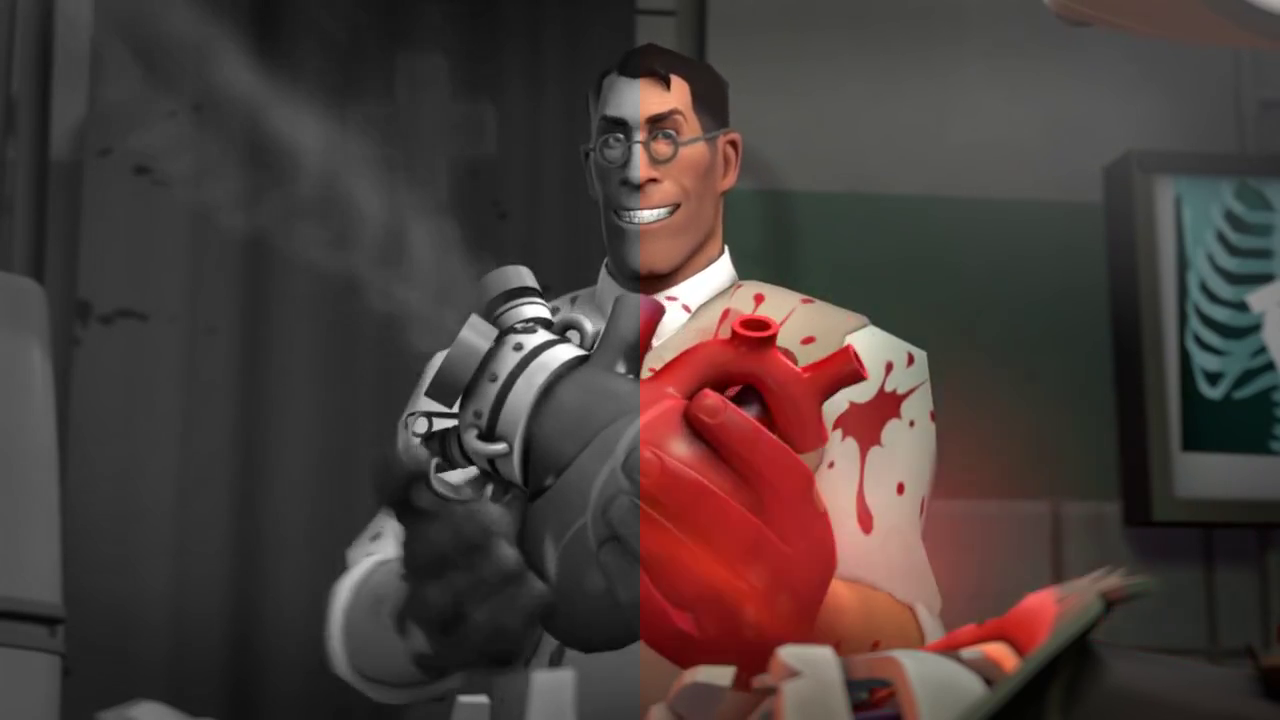
\includegraphics[width=11cm,keepaspectratio]{pics/rgb_gray.png}
  \end{figure}
  \url{https://www.youtube.com/watch?v=36lSzUMBJnc}
\end{frame}



\begin{frame}[fragile]
\frametitle{Thresholding}
  {\scriptsize
  \begin{minted}[frame=lines]{glsl}
#version 450

layout(location=0)out vec4 fColor;

layout(binding=0)uniform sampler2D frame;

//texture coordinates
in vec2 vCoord;

uniform uvec2 windowSize = uvec2(1,1);

void main(){
  //read from texture
  vec3 color = texture(frame,vCoord).xyz;

  //convertex to intensity
  float intensity = dot(vec3(.2126,.7152,.0722),color);

  //write intensity to framebuffer
  fColor = vec4(intensity>.4);
}
  \end{minted}
  }
\end{frame}

\begin{frame}
\frametitle{Example - thresholding}
  \begin{figure}[h]
  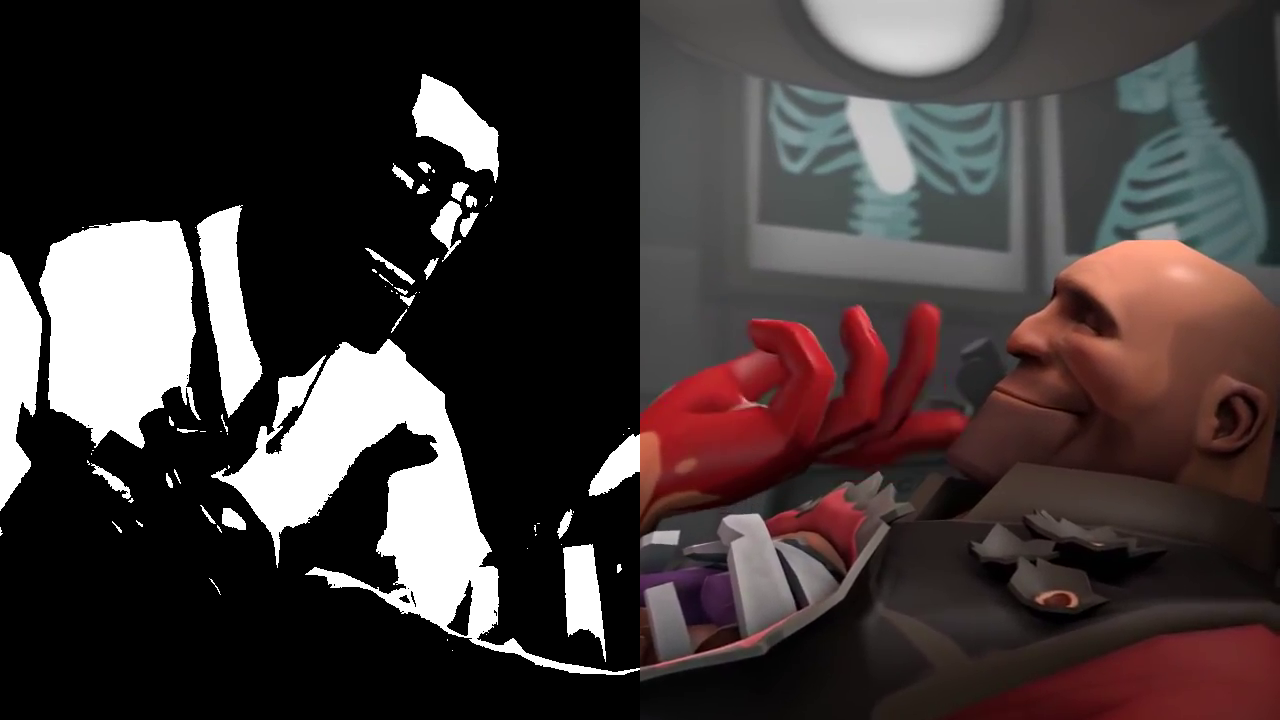
\includegraphics[width=11cm,keepaspectratio]{pics/rgb_thresholding.png}
  \end{figure}
  \url{https://www.youtube.com/watch?v=36lSzUMBJnc}
\end{frame}



\begin{frame}[fragile]
\frametitle{Red extraction}
  {\scriptsize
  \begin{minted}[frame=lines]{glsl}
#version 450

layout(location=0)out vec4 fColor;

layout(binding=0)uniform sampler2D frame;

//texture coordinates
in vec2 vCoord;

uniform uvec2 windowSize = uvec2(1,1);

void main(){
  //read from texture
  vec3 color = texture(frame,vCoord).xyz;

  float redness = 1-distance(color.rbg,vec3(1,0,0))/sqrt(3);

  //convertex to intensity
  float intensity = dot(vec3(.2126,.7152,.0722),color);

  //write color to framebuffer
  fColor = vec4(mix(vec3(intensity>0.4),redGradient(intensity).xyz,
    smoothstep(0.6,.8,redness,1)),1);
}
  \end{minted}
  }
\end{frame}

\begin{frame}
\frametitle{Example - red extraction}
  \begin{figure}[h]
  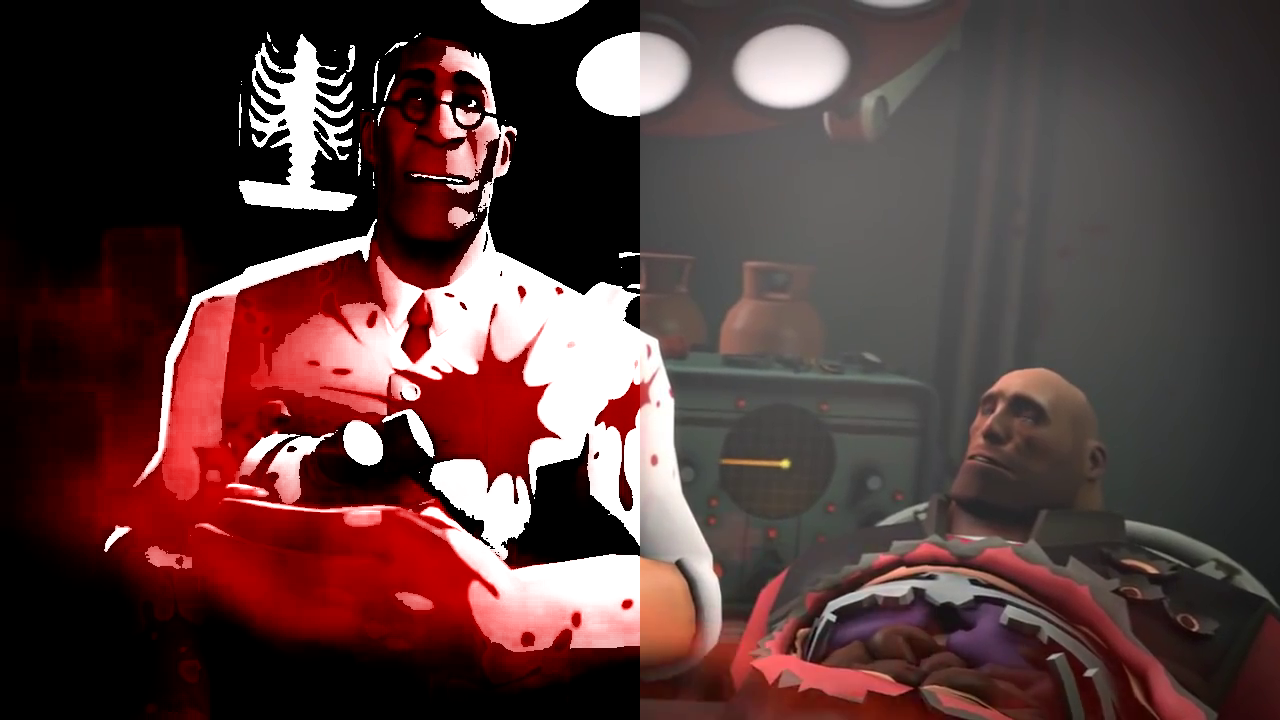
\includegraphics[width=11cm,keepaspectratio]{pics/red_extraction.png}
  \end{figure}
  \url{https://www.youtube.com/watch?v=36lSzUMBJnc}
\end{frame}




\begin{frame}[fragile]
\frametitle{Edge detection - sobel}
  {\scriptsize
  \begin{minted}[frame=lines]{glsl}
#version 450
...
void main(){
  //read from texture
  float intensities[9];

  for(int y=-1;y<=1;++y)
    for(int x=-1;x<=1;++x)
      intensities[(1+y)*3+(1+x)] = 
        dot(vec3(.2126,.7152,.0722),texelFetch(frame,texelCoord+ivec2(x,y),0).xyz);

  vec3 color = texelFetch(frame,texelCoord,0).xyz;

  float xSobelMask[9] = {-1,0,1,-2,0,2,-1,0,1};
  float ySobelMask[9] = {-1,-2,-1,0,0,0,1,2,1};

  float xSobel = 0;
  float ySobel = 0;

  for(int i=0;i<9;++i){
    xSobel += intensities[i]*xSobelMask[i];
    ySobel += intensities[i]*ySobelMask[i];
  }

  vec3 sobel = vec3(length(vec2(xSobel,ySobel)));
  
  fColor = vec4(sobel,1);
}
  \end{minted}
  }
\end{frame}

\begin{frame}
\frametitle{Example - sobel filter}
  \begin{figure}[h]
  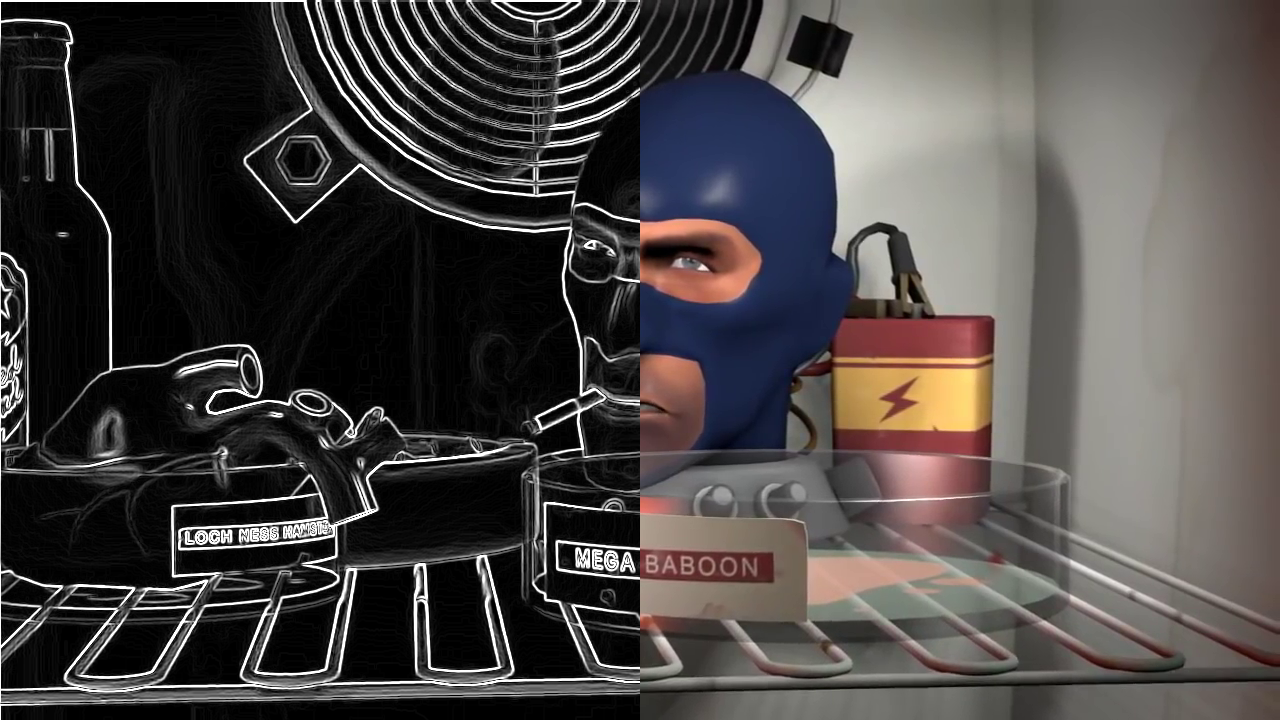
\includegraphics[width=11cm,keepaspectratio]{pics/sobel.png}
  \end{figure}
  \url{https://www.youtube.com/watch?v=36lSzUMBJnc}
\end{frame}

\begin{frame}[fragile]
\frametitle{Gaussian blur}
  {\scriptsize
  \begin{minted}[frame=lines]{glsl}
#version 450

float gaussFunction(float x,float sigma){
  return inversesqrt(2*radians(180)*sigma*sigma)*exp(-x*x/(2*sigma*sigma));
}

void main(){

  const int gaussSize = 10;
  vec3 gauss = vec3(0);
  float accumulatedWeights = 0;
  for(int x=-gaussSize;x<=gaussSize;++x)
    for(int y=-gaussSize;y<=gaussSize;++y){
      float distanceFromCenter = length(vec2(x,y));
      float g = gaussFunction(distanceFromCenter,10);
      accumulatedWeights += g;
      gauss += texelFetch(frame,texelCoord+ivec2(x,y),0).xyz*g;
    }
  gauss /= accumulatedWeights;

  fColor = vec4(gauss,1);
}
  \end{minted}
  }
\end{frame}

\begin{frame}
\frametitle{Example - gaussian blur}
  \begin{figure}[h]
  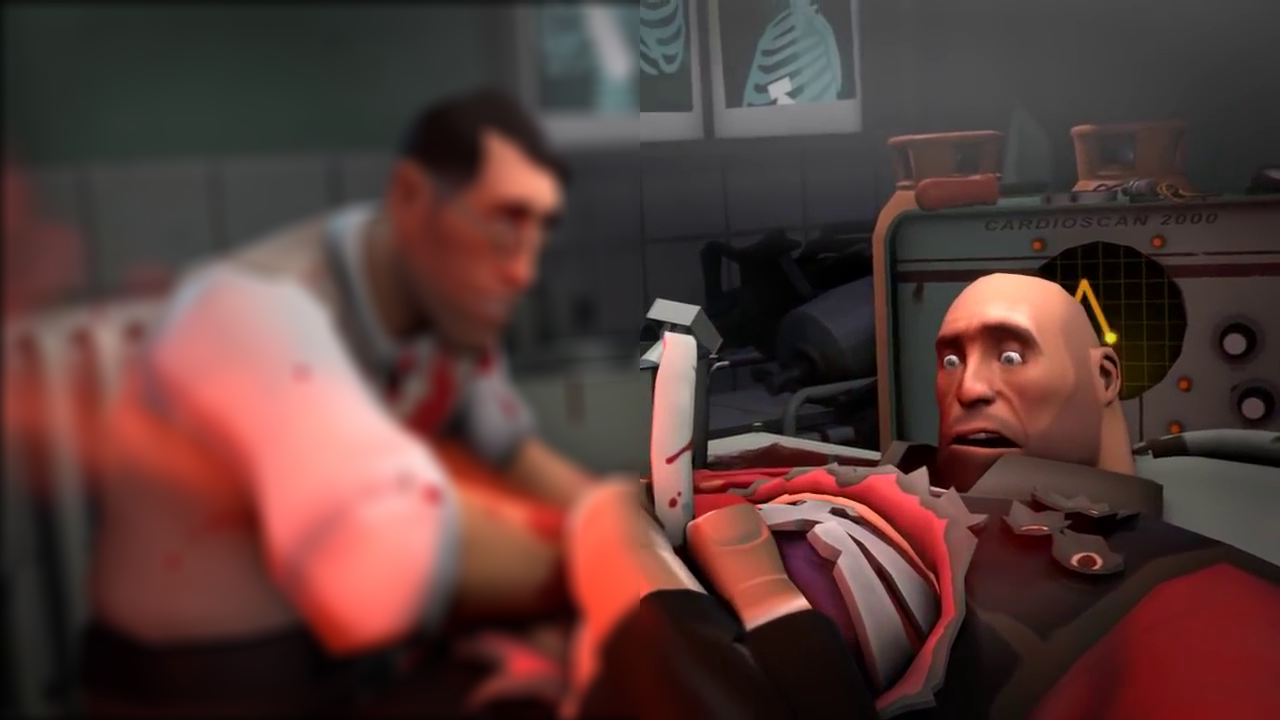
\includegraphics[width=11cm,keepaspectratio]{pics/gauss.png}
  \end{figure}
  \url{https://www.youtube.com/watch?v=36lSzUMBJnc}
\end{frame}

\begin{frame}
  \frametitle{Example - sin(x) function aplied to intensity}
  \begin{figure}[h]
  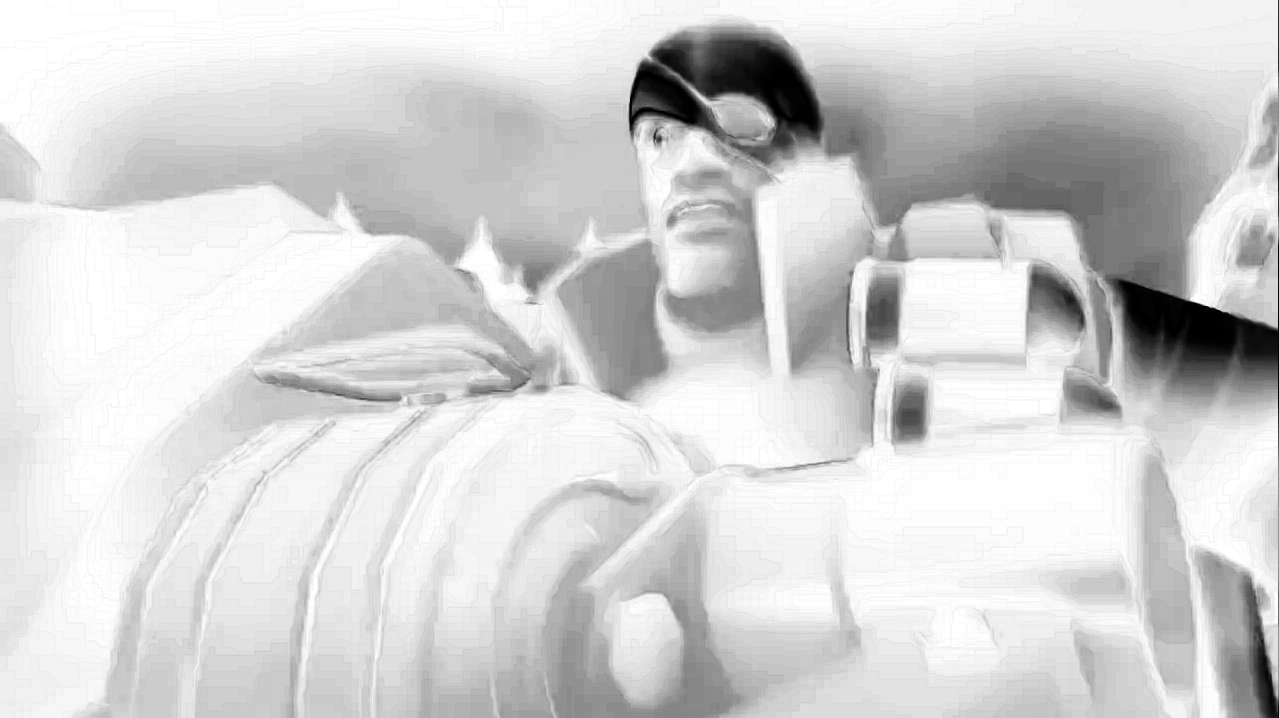
\includegraphics[width=11cm,keepaspectratio]{pics/sin.png}
  \end{figure}
  \url{https://www.youtube.com/watch?v=36lSzUMBJnc}
\end{frame}

